% Homework Template
\documentclass[a4paper]{article}
\usepackage{ctex}
\usepackage{amsmath, amssymb, amsthm}
\usepackage{moreenum}
\usepackage{mathtools}
\usepackage{url}
\usepackage{bm}
\usepackage{enumitem}
\usepackage{graphicx}
\usepackage{subcaption}
\usepackage{booktabs} % toprule
\usepackage[mathcal]{eucal}
\usepackage[thehwcnt = 6]{iidef}
\usepackage{float}

\usepackage[sort]{natbib}

\thecourseinstitute{清华大学电子工程系}
\thecoursename{\textbf{媒体与认知} \space 课堂2}
\theterm{2021-2022学年春季学期}
\hwname{作业}

\begin{document}
\courseheader{}
\name{李智毅}
\vspace{3mm}
\centerline{\textbf{\Large{调研报告部分}}}
\vspace{3mm}

\section{调研报告}

\textbf{背景介绍}\\
\hspace{2em}2019年底,一场新冠肺炎席卷全球。如今随着疫情不断常态化发展,如何准确检测识别新冠患者是一个十分重要的问题。
常规的检测手段是利用核酸、抗原检测,然而它们都有一定的误检率,难以准确分辨普通流感和新冠肺炎,这在一定程度上妨碍了有效的管控。
因此,需要研究新的数据与分析方法,进而准确识别新冠感染患者。\\
\hspace{2em}对于新冠肺炎,可以利用其在影像学数据(如肺部CT)上的特征体现进行鉴别。然而由于各种肺炎在影像学上的特征差异不明显,依靠当前的经典检测手段仍难以准确鉴别。
因此,我们希望能够通过机器学习的方法进行图像处理,通过已有的影像学数据训练分类器,在实际诊断中能够为医师提供参考,提升识别准确率。\\

\textbf{解决措施}\\
\hspace{2em}通过对患者影像学数据进行学习,可以构建分类器以鉴别新冠肺炎。现有解决方法包括传统机器学习(\cite{tianbin})、深度学习(\cite{xucuilian}, \cite{zouwenwen})等方法。\\
\hspace{2em}\cite{tianbin} 研究基于传统机器学习辅助诊断展开,利用较少的数据进行学习分析。
他们对比了14种机器学习模型进行预测,包括线性支持向量机分类器、增强学习分类器、逻辑回归分类器、决策树分类器等,给出了不同模型的受试者工作特征曲线(ROC)及曲线下面积(AUC),并将AUC作为评价模型性能的指标(以上AUC均处于90\%至95\%之间不等)。
由此可见,此类传统机器方法获得的准确率较好,对辅助诊断具有现实意义。\\
\hspace{2em}\cite{zouwenwen} 应用深度学习对影像学资料展开研究,基于VGGNet和ResNet网络,根据BIMCV COVID-19+数据集进行训练。
整体分类器模型包括CNN(VGGNet或ResNet)及可视化(Score-CAM)。
达到的准确率分别为95.56\%(VGGNet)、98.89\%(ResNet),对于该问题的分类有效。\\

\textbf{效果分析}\\
\hspace{2em}基于机器学习对影像学数据分析的方法主要包括传统机器学习及深度学习等。
其中传统机器学习方法在较少的数据集下进行训练,对不同的分类模型给出了相应的结果;深度学习采用了常用网络结构VGGNet及ResNet结构,取得了较好的准确率。\\

\textbf{未来思路}\\
\hspace{2em}可以看到,现有的研究方法于模型对于实现准确的预测仍有一定差距,需要继续提升。
主要包含以下原因:有效数据量较小,难以获得准确的模型参数;当前模型解释性较差,可以进一步研究影像学特征设计相应的机器学习算法等。
因此,之后的研究工作可以首先采取数据增强、增大样本数等方式获取更多数据,同时研究分析影像学特征提出对应模型。\\

\vspace{3mm}
\centerline{\textbf{\Large{编程部分}}}
\vspace{3mm}
% 请根据是否选择自选课题的情况选择“编程作业报告”或“自选课题开题报告”中的一项完成
\section{编程作业报告}
\subsection{完成Transformer场景文本识别任务的程序代码}
按照要求搭建Transformer的结构,以及网络结构和测试代码,运行“network.py”验证网络结构,结果(如图1所示):\\
显示“The output size of model is correct!”
\begin{figure}[H]
    \centering
    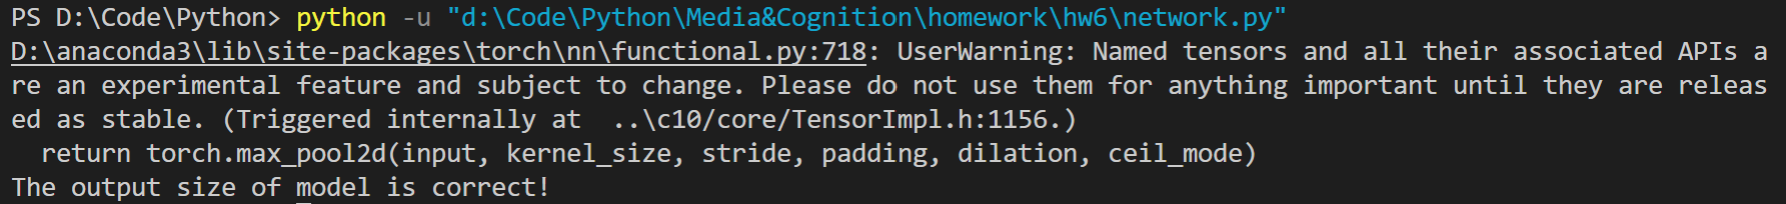
\includegraphics[width=12cm]{Fig_1.png}
    \caption{测试网络输出维度}
\end{figure}

\subsection{训练、预测、可视化}
\subsubsection{模型的训练与验证}
使用默认参数训练,输入"python main.py --mode train",有训练结果如下:(loss及验证集曲线如图2所示)\\
\begin{figure}
    \centering
    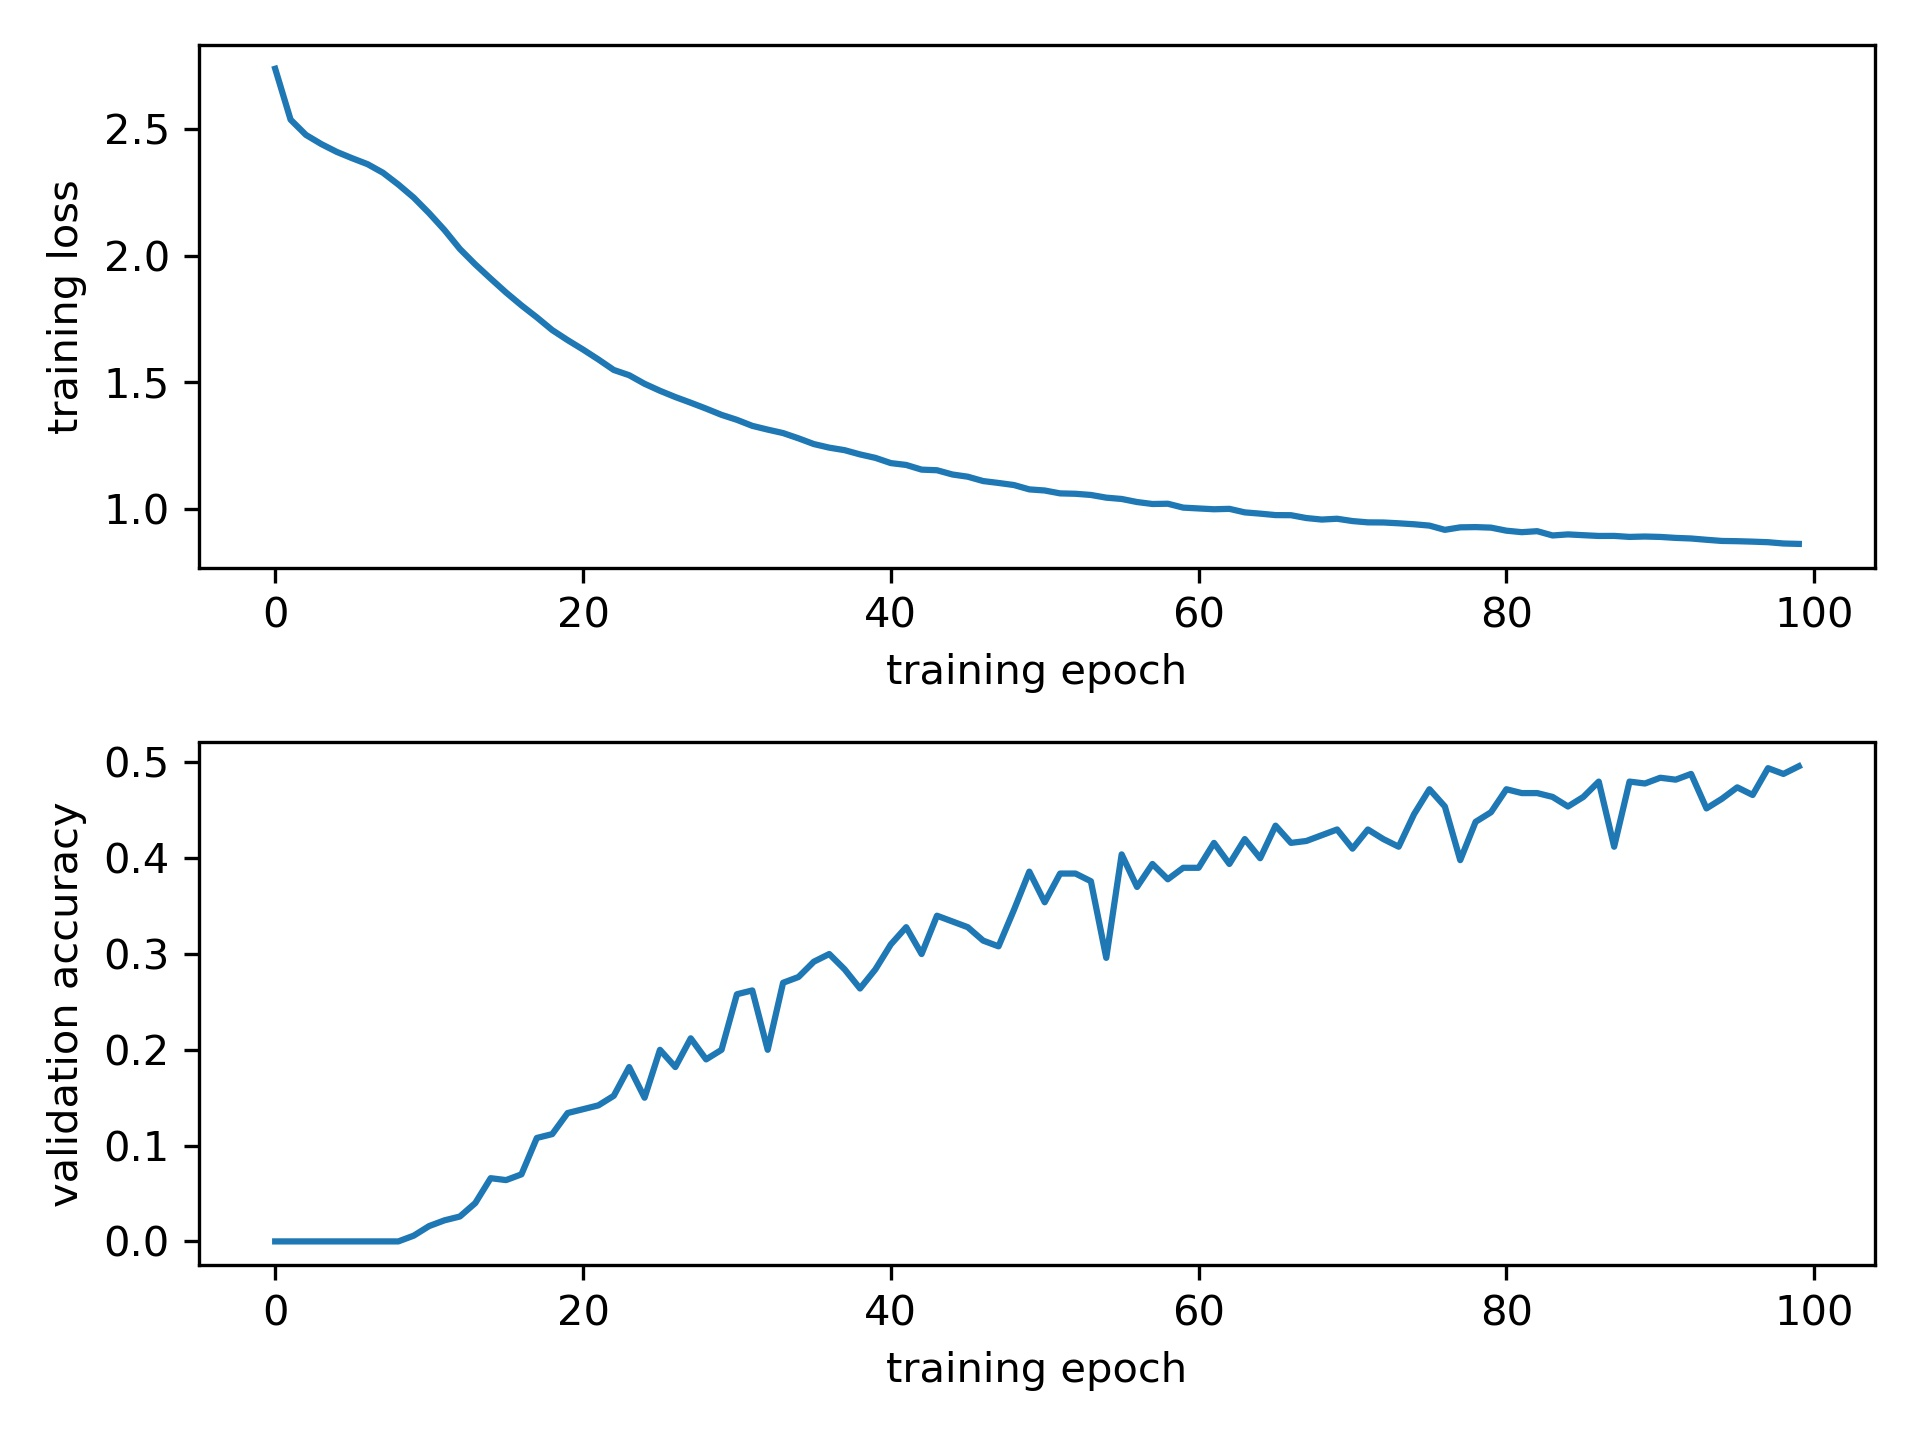
\includegraphics[width=12cm]{loss_and_accuracy.jpg}
    \caption{loss及验证集准确率曲线}
\end{figure}
训练轮数:epoch=100 \\
测试集准确率:49\% \\

\subsubsection{使用训练好的模型预测新的文本图像}
使用训练100轮之后的模型预测所给的两个图像,有结果如下:\\
对于parking:(如图3) \\
\begin{figure}
    \centering
    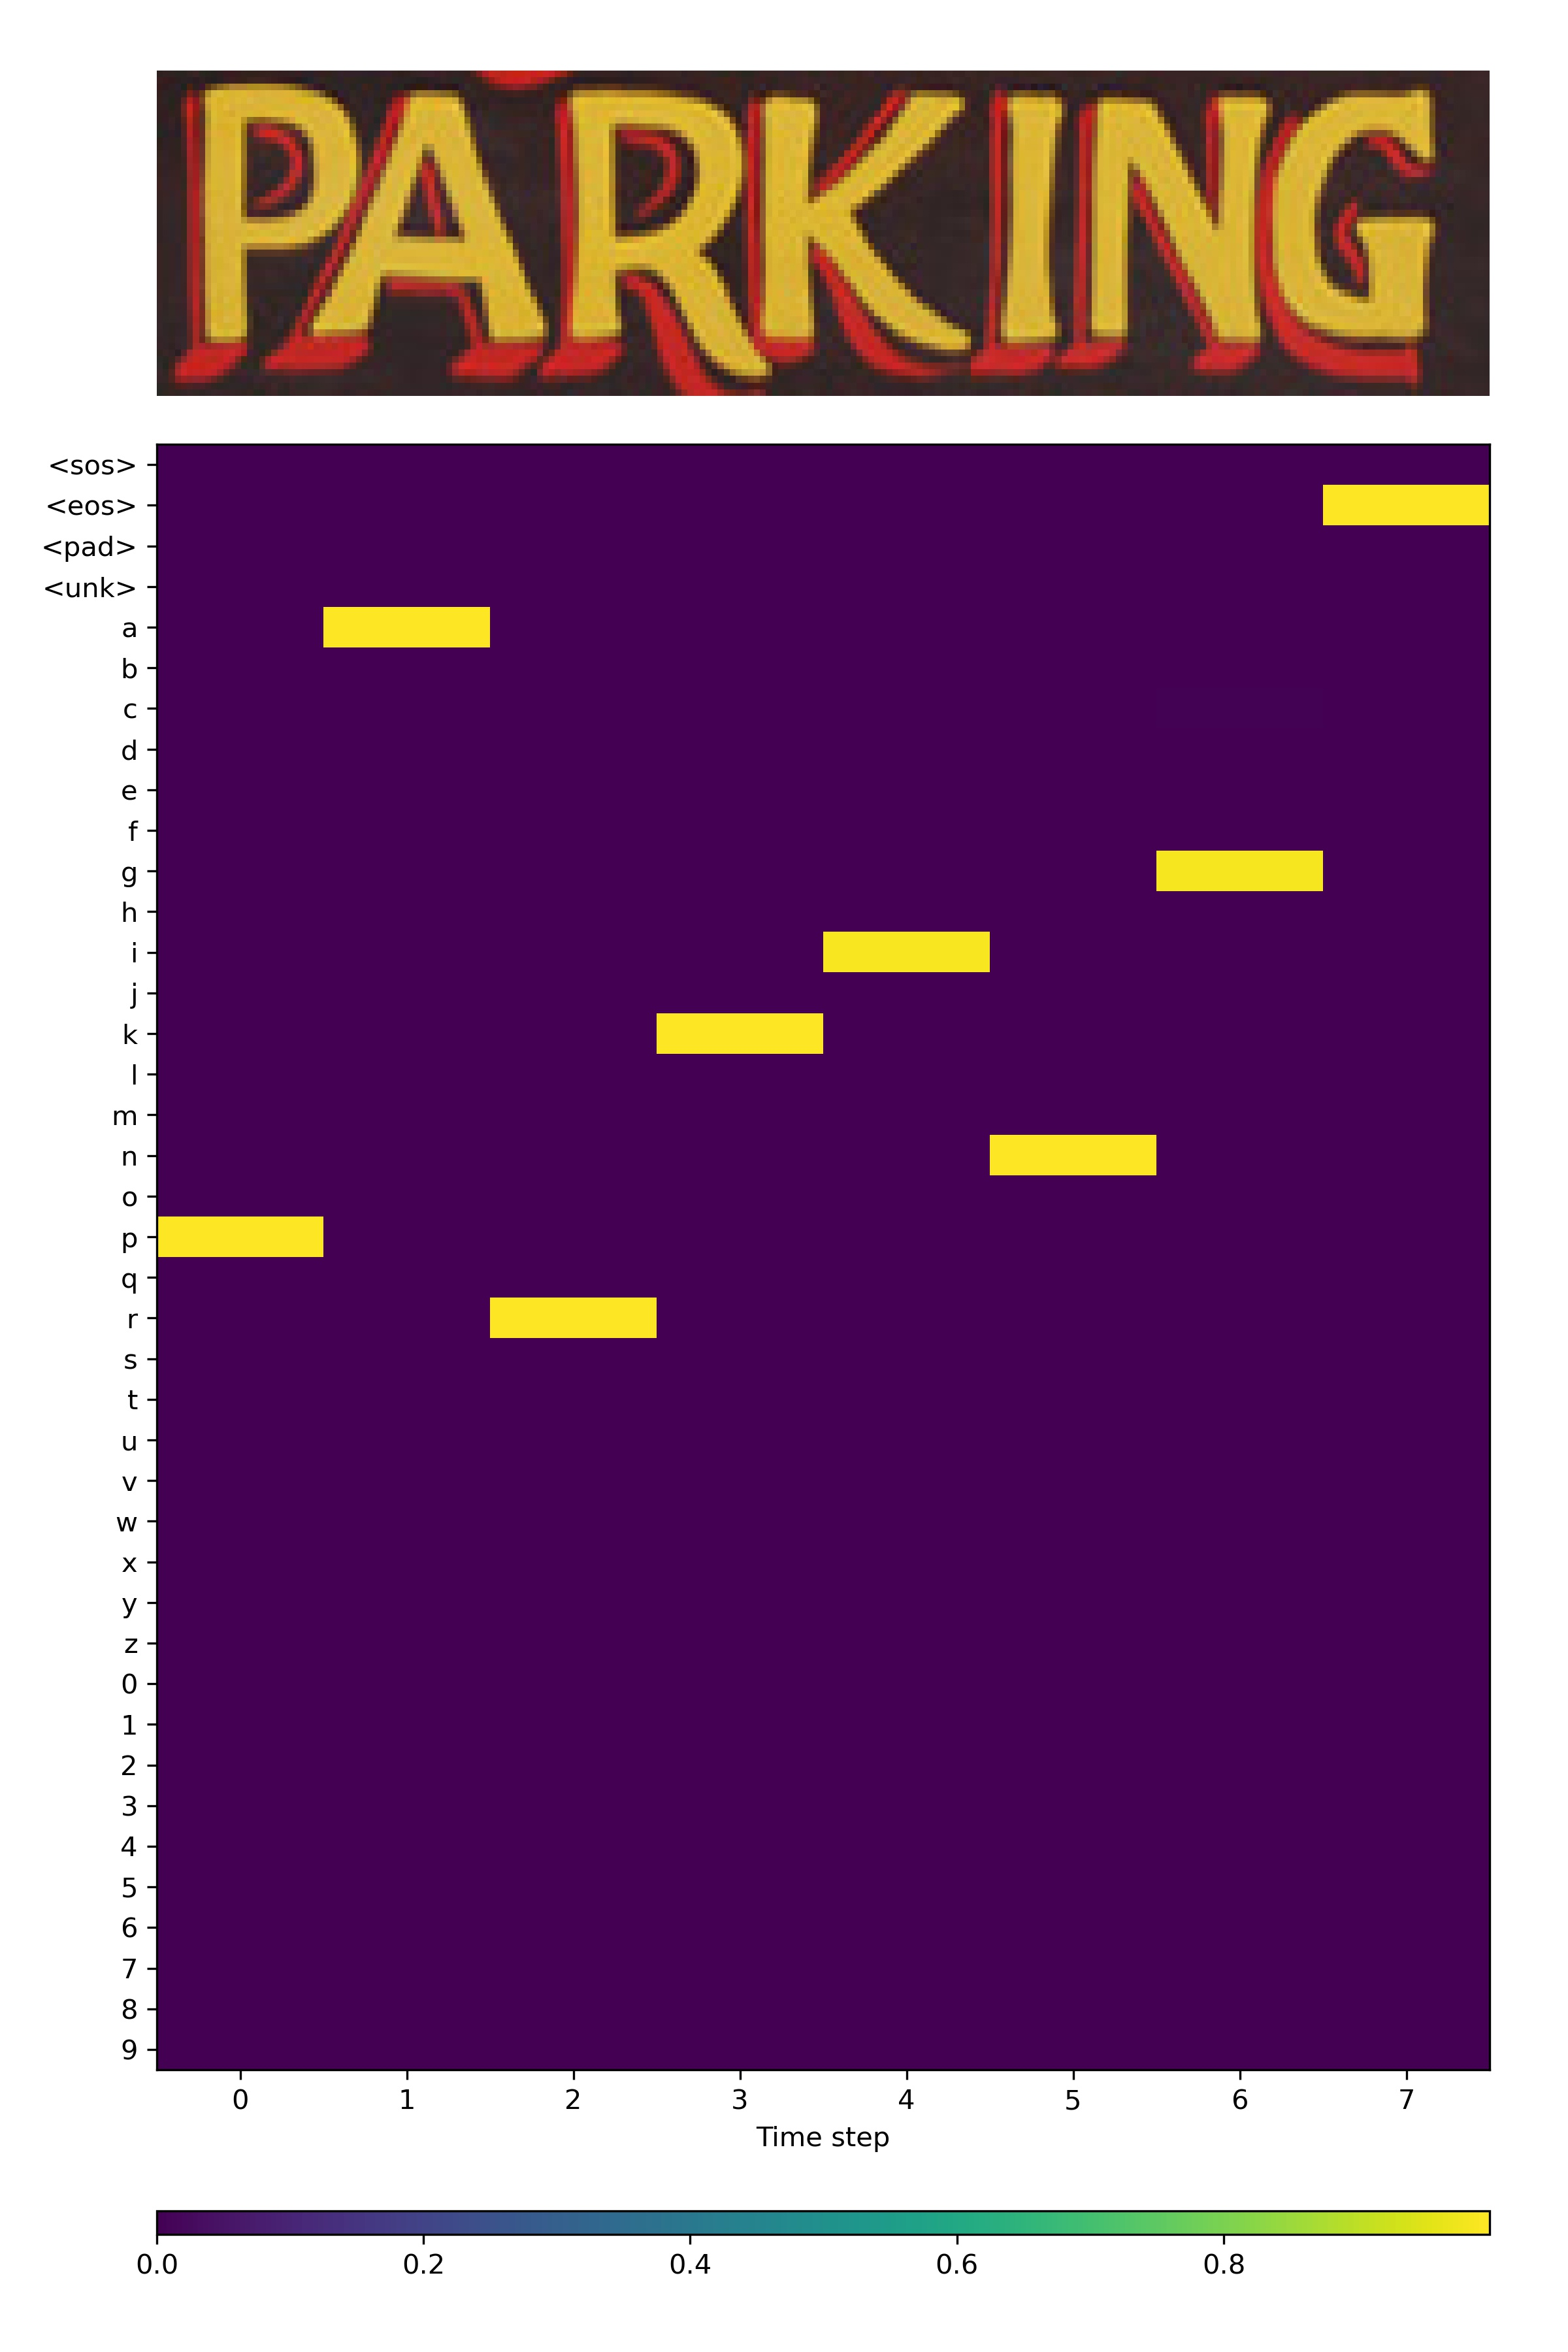
\includegraphics[width=12cm]{parking_vis.jpg}
    \caption{parking预测结果}
\end{figure}
输入文本:parking \\
预测文本:parking \\
对于recommend:(如图4)
\begin{figure}
    \centering
    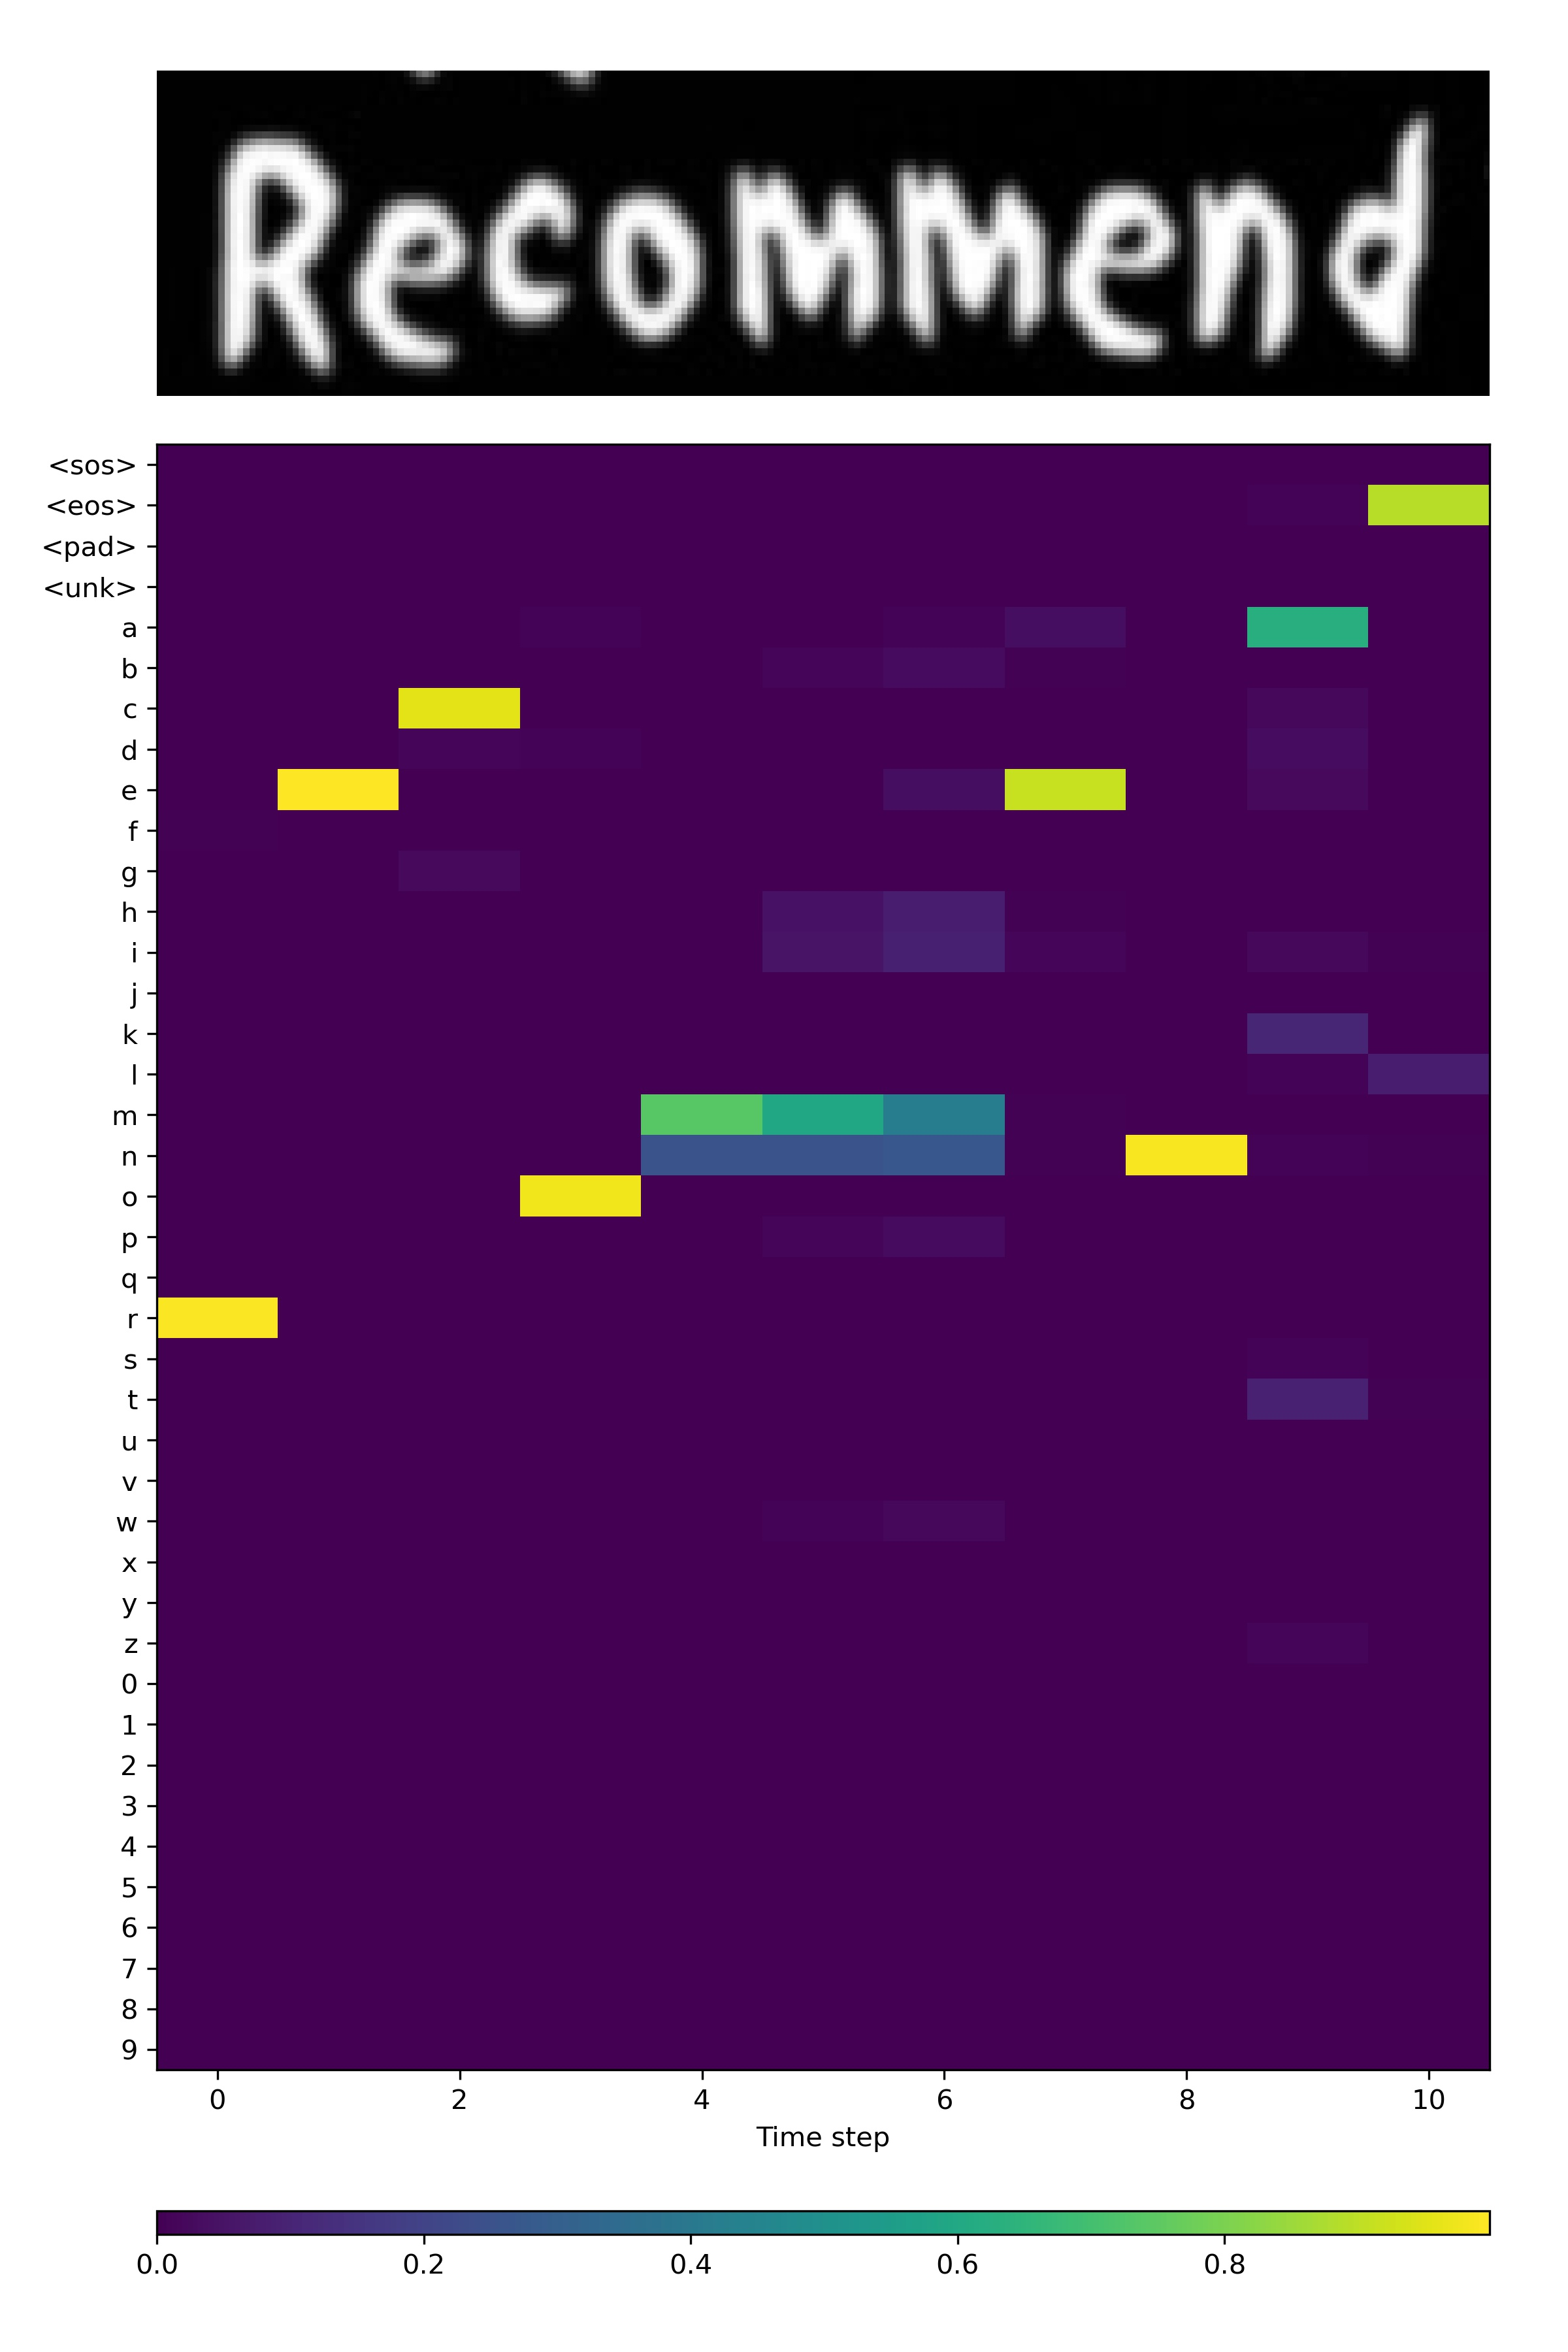
\includegraphics[width=12cm]{recommend_vis.jpg}
    \caption{recommend预测结果}
\end{figure}
输入文本:recommend \\
预测文本:recommena \\

可以看见,所训练模型对于大部分识别任务能够较好完成,两次测试中仅在recommend中将最后一个字母识别出错,可以接受。\\
从图中可以看到,该模型对parking预测置信度较高,而对相对不那么规整的recommend在O、M、N、D几个字母上显示都有一定的误差。\\

\subsection{结果分析}
\subsubsection{Transformer具有并行训练特性的原因}
由于引入注意力掩码M,使得当前解码时刻与之后无关,因此实现并行计算。\\
\subsubsection{Transformer与CTC解码的区别及原因}
Transformer解码的特点:由隐含层及前时刻的输出依次得到当前输出结果,直接生成解码序列。\\
CTC解码的特点:得到由序列的预测结果以及空白字符'-'组成的序列,以此按照其规则输出序列。\\
产生区别的原因:CTC使用RNN结构,将序列分割成小部分,每一部分按照概率预测可能结果。因此CTC终止根据空白字符的出现;
而Transformer使用注意力机制,利用Encoder-Decoder方式,解码根据前一时刻结果与隐含层状态输出。Transformer的终止根据预测出结束符。\\


\bibliographystyle{thuthesis-numeric}
\bibliography{refs}  % 参考文献使用 BibTeX 编译

\end{document}



%%% Local Variables:
%%% mode: late\rvx
%%% TeX-master: t
%%% End:
